\subsection{GMREDI: Gent/McWiliams/Redi SGS Eddy Parameterization}
\label{sec:pkg:gmredi}
\begin{rawhtml}
<!-- CMIREDIR:gmredi: -->
\end{rawhtml}

There are two parts to the Redi/GM parameterization of geostrophic
eddies. The first aims to mix tracer properties along isentropes
(neutral surfaces) by means of a diffusion operator oriented along the
local isentropic surface (Redi). The second part, adiabatically
re-arranges tracers through an advective flux where the advecting flow
is a function of slope of the isentropic surfaces (GM).

The first GCM implementation of the Redi scheme was by Cox 1987 in the
GFDL ocean circulation model. The original approach failed to
distinguish between isopycnals and surfaces of locally referenced
potential density (now called neutral surfaces) which are proper
isentropes for the ocean. As will be discussed later, it also appears
that the Cox implementation is susceptible  to a computational mode.
Due to this mode, the Cox scheme requires a background lateral
diffusion to be present to conserve the integrity of the model fields.

The GM parameterization was then added to the GFDL code in the form of
a non-divergent bolus velocity. The method defines two
stream-functions expressed in terms of the isoneutral slopes subject
to the boundary condition of zero value on upper and lower
boundaries. The horizontal bolus velocities are then the vertical
derivative of these functions. Here in lies a problem highlighted by
Griffies et al., 1997: the bolus velocities involve multiple
derivatives on the potential density field, which can consequently
give rise to noise. Griffies et al. point out that the GM bolus fluxes
can be identically written as a skew flux which involves fewer
differential operators. Further, combining the skew flux formulation
and Redi scheme, substantial cancellations take place to the point
that the horizontal fluxes are unmodified from the lateral diffusion
parameterization.

\subsubsection{Redi scheme: Isopycnal diffusion}

The Redi scheme diffuses tracers along isopycnals and introduces a
term in the tendency (rhs) of such a tracer (here $\tau$) of the form:
\begin{equation}
\bf{\nabla} \cdot \kappa_\rho \bf{K}_{Redi}  \bf{\nabla} \tau
\end{equation}
where $\kappa_\rho$ is the along isopycnal diffusivity and
$\bf{K}_{Redi}$ is a rank 2 tensor that projects the gradient of
$\tau$ onto the isopycnal surface. The unapproximated projection tensor is:
\begin{equation}
\bf{K}_{Redi} = \left(
\begin{array}{ccc}
1 + S_x& S_x S_y & S_x \\
S_x S_y  & 1 + S_y & S_y \\
S_x & S_y & |S|^2 \\
\end{array}
\right)
\end{equation}
Here, $S_x = -\partial_x \sigma / \partial_z \sigma$ and $S_y =
-\partial_y \sigma / \partial_z \sigma$ are the components of the
isoneutral slope.

The first point to note is that a typical slope in the ocean interior
is small, say of the order $10^{-4}$. A maximum slope might be of
order $10^{-2}$ and only exceeds such in unstratified regions where
the slope is ill defined. It is therefore justifiable, and
customary, to make the small slope approximation, $|S| << 1$. The Redi
projection tensor then becomes:
\begin{equation}
\bf{K}_{Redi} = \left(
\begin{array}{ccc}
1 & 0 & S_x \\
0 & 1 & S_y \\
S_x & S_y & |S|^2 \\
\end{array}
\right)
\end{equation}


\subsubsection{GM parameterization}

The GM parameterization aims to parameterise the ``advective'' or
``transport'' effect of geostrophic eddies by means of a ``bolus''
velocity, $\bf{u}^*$. The divergence of this advective flux is added
to the tracer tendency equation (on the rhs):
\begin{equation}
- \bf{\nabla} \cdot \tau \bf{u}^*
\end{equation}

The bolus velocity is defined as:
\begin{eqnarray}
u^* & = & - \partial_z F_x \\
v^* & = & - \partial_z F_y \\
w^* & = & \partial_x F_x + \partial_y F_y
\end{eqnarray}
where $F_x$ and $F_y$ are stream-functions with boundary conditions
$F_x=F_y=0$ on upper and lower boundaries. The virtue of casting the
bolus velocity in terms of these stream-functions is that they are
automatically non-divergent ($\partial_x u^* + \partial_y v^* = -
\partial_{xz} F_x - \partial_{yz} F_y = - \partial_z w^*$). $F_x$ and
$F_y$ are specified in terms of the isoneutral slopes $S_x$ and $S_y$:
\begin{eqnarray}
F_x & = & \kappa_{GM} S_x \\
F_y & = & \kappa_{GM} S_y
\end{eqnarray}
This is the form of the GM parameterization as applied by Donabasaglu,
1997, in MOM versions 1 and 2.

\subsubsection{Griffies Skew Flux}

Griffies notes that the discretisation of bolus velocities involves
multiple layers of differencing and interpolation that potentially
lead to noisy fields and computational modes. He pointed out that the
bolus flux can be re-written in terms of a non-divergent flux and a
skew-flux:
\begin{eqnarray*}
\bf{u}^* \tau
& = &
\left( \begin{array}{c}
- \partial_z ( \kappa_{GM} S_x ) \tau \\
- \partial_z ( \kappa_{GM} S_y ) \tau \\
(\partial_x \kappa_{GM} S_x + \partial_y \kappa_{GM} S_y)\tau
\end{array} \right)
\\
& = &
\left( \begin{array}{c}
- \partial_z ( \kappa_{GM} S_x \tau) \\
- \partial_z ( \kappa_{GM} S_y \tau) \\
\partial_x ( \kappa_{GM} S_x \tau) + \partial_y ( \kappa_{GM} S_y) \tau)
\end{array} \right)
+ \left( \begin{array}{c}
 \kappa_{GM} S_x \partial_z \tau \\
 \kappa_{GM} S_y \partial_z \tau \\
- \kappa_{GM} S_x \partial_x \tau - \kappa_{GM} S_y) \partial_y \tau
\end{array} \right)
\end{eqnarray*}
The first vector is non-divergent and thus has no effect on the tracer
field and can be dropped. The remaining flux can be written:
\begin{equation}
\bf{u}^* \tau = - \kappa_{GM} \bf{K}_{GM} \bf{\nabla} \tau
\end{equation}
where
\begin{equation}
\bf{K}_{GM} =
\left(
\begin{array}{ccc}
0 & 0 & -S_x \\
0 & 0 & -S_y \\
S_x & S_y & 0
\end{array}
\right)
\end{equation}
is an anti-symmetric tensor.

This formulation of the GM parameterization involves fewer derivatives
than the original and also involves only terms that already appear in
the Redi mixing scheme. Indeed, a somewhat fortunate cancellation
becomes apparent when we use the GM parameterization in conjunction
with the Redi isoneutral mixing scheme:
\begin{equation}
\kappa_\rho \bf{K}_{Redi} \bf{\nabla} \tau
- u^* \tau = 
( \kappa_\rho \bf{K}_{Redi} + \kappa_{GM} \bf{K}_{GM} ) \bf{\nabla} \tau
\end{equation}
In the instance that $\kappa_{GM} = \kappa_{\rho}$ then
\begin{equation}
\kappa_\rho \bf{K}_{Redi} + \kappa_{GM} \bf{K}_{GM} =
\kappa_\rho
\left( \begin{array}{ccc}
1 & 0 & 0 \\
0 & 1 & 0 \\
2 S_x & 2 S_y & |S|^2 
\end{array}
\right)
\end{equation}
which differs from the variable Laplacian diffusion tensor by only
two non-zero elements in the $z$-row.

\fbox{ \begin{minipage}{4.75in}
{\em S/R GMREDI\_CALC\_TENSOR} ({\em pkg/gmredi/gmredi\_calc\_tensor.F})

$\sigma_x$: {\bf SlopeX} (argument on entry)

$\sigma_y$: {\bf SlopeY} (argument on entry)

$\sigma_z$: {\bf SlopeY} (argument)

$S_x$: {\bf SlopeX} (argument on exit)

$S_y$: {\bf SlopeY} (argument on exit)

\end{minipage} }



\subsubsection{Variable $\kappa_{GM}$}

Visbeck et al., 1996, suggest making the eddy coefficient,
$\kappa_{GM}$, a function of the Eady growth rate,
$|f|/\sqrt{Ri}$. The formula involves a non-dimensional constant,
$\alpha$, and a length-scale $L$:
\begin{displaymath}
\kappa_{GM} = \alpha L^2 \overline{ \frac{|f|}{\sqrt{Ri}} }^z
\end{displaymath}
where the Eady growth rate has been depth averaged (indicated by the
over-line). A local Richardson number is defined $Ri = N^2 / (\partial
u/\partial z)^2$ which, when combined with thermal wind gives:
\begin{displaymath}
\frac{1}{Ri} = \frac{(\frac{\partial u}{\partial z})^2}{N^2} =
\frac{ ( \frac{g}{f \rho_o} | {\bf \nabla} \sigma | )^2 }{N^2} =
\frac{ M^4 }{ |f|^2 N^2 }
\end{displaymath}
where $M^2$ is defined $M^2 = \frac{g}{\rho_o} |{\bf \nabla} \sigma|$.
Substituting into the formula for $\kappa_{GM}$ gives:
\begin{displaymath}
\kappa_{GM} = \alpha L^2 \overline{ \frac{M^2}{N} }^z =
\alpha L^2 \overline{ \frac{M^2}{N^2} N }^z =
\alpha L^2 \overline{ |S| N }^z
\end{displaymath}


\subsubsection{Tapering and stability}

Experience with the GFDL model showed that the GM scheme has to be
matched to the convective parameterization. This was originally
expressed in connection with the introduction of the KPP boundary
layer scheme (Large et al., 97) but in fact, as subsequent experience
with the MIT model has found, is necessary for any convective
parameterization.

\fbox{ \begin{minipage}{4.75in}
{\em S/R GMREDI\_SLOPE\_LIMIT} ({\em
pkg/gmredi/gmredi\_slope\_limit.F})

$\sigma_x, s_x$: {\bf SlopeX} (argument)

$\sigma_y, s_y$: {\bf SlopeY} (argument)

$\sigma_z$: {\bf dSigmadRReal} (argument)

$z_\sigma^{*}$: {\bf dRdSigmaLtd} (argument)

\end{minipage} }

\begin{figure}
\begin{center}
\resizebox{5.0in}{3.0in}{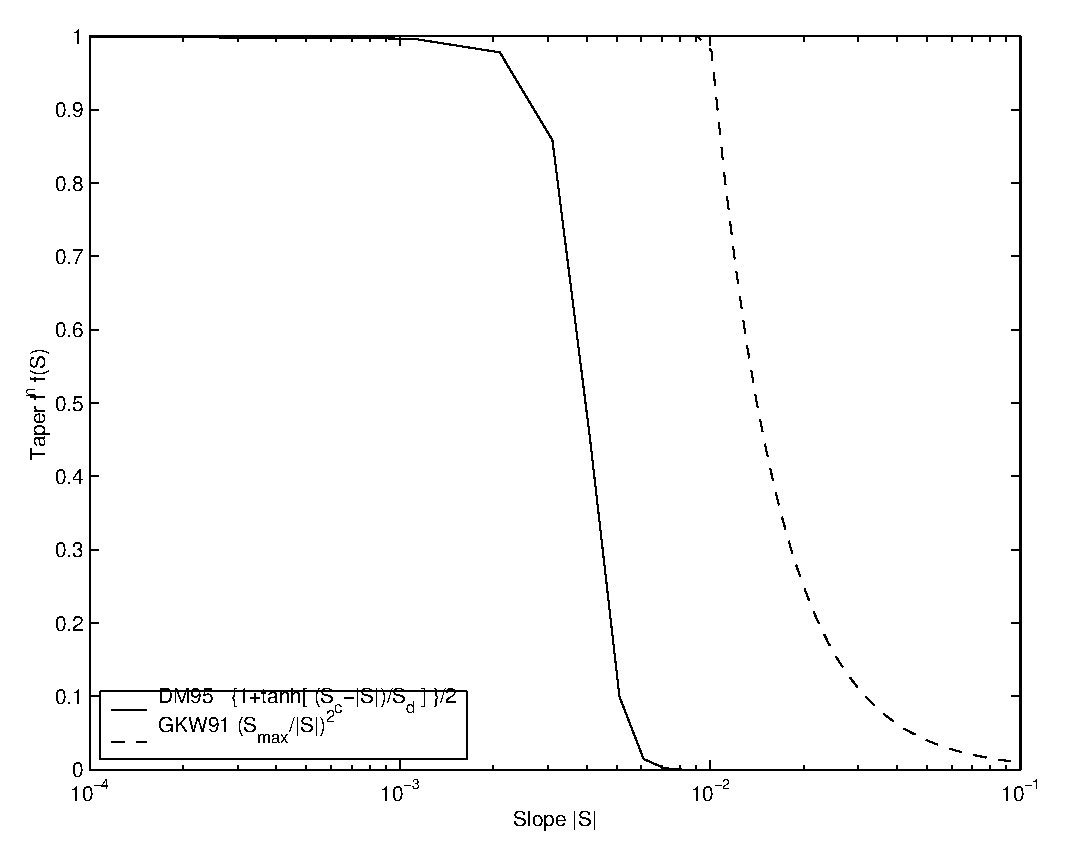
\includegraphics{part6/tapers.eps}}
\end{center}
\caption{Taper functions used in GKW99 and DM95.}
\label{fig:tapers}
\end{figure}

\begin{figure}
\begin{center}
\resizebox{5.0in}{3.0in}{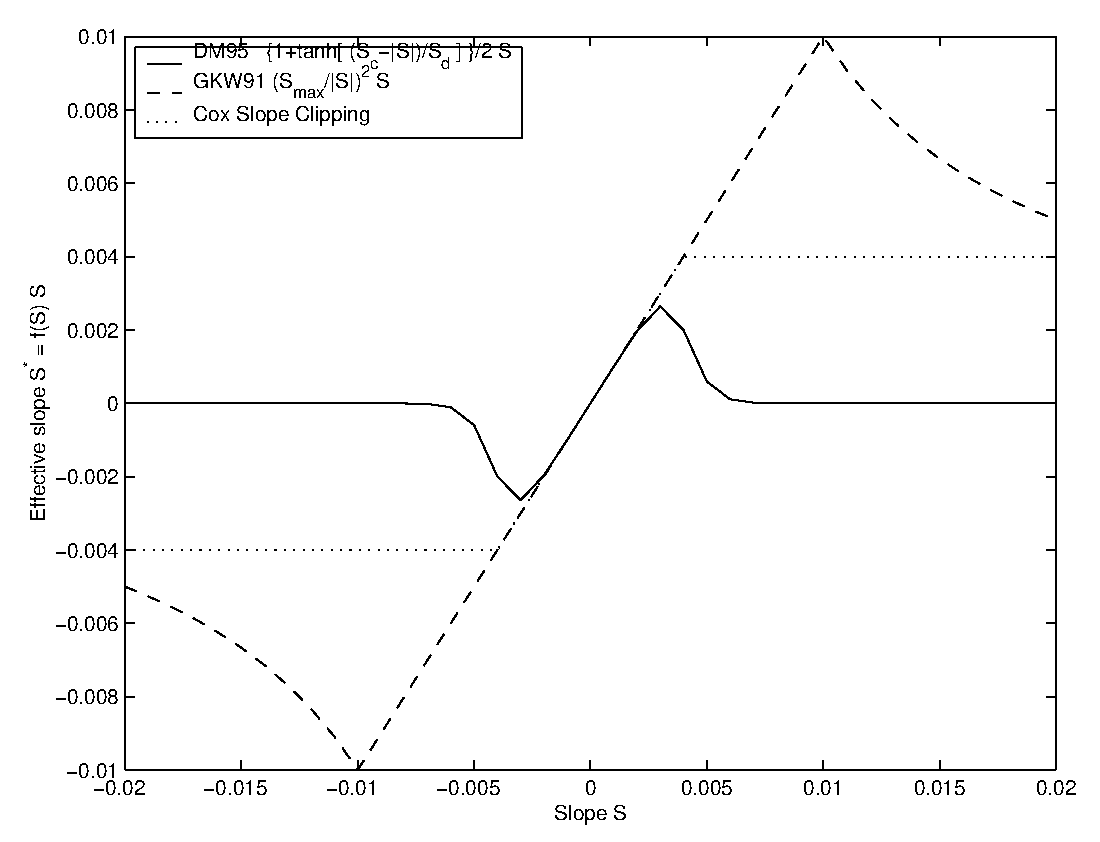
\includegraphics{part6/effective_slopes.eps}}
\end{center}
\caption{Effective slope as a function of ``true'' slope using Cox
slope clipping, GKW91 limiting and DM95 limiting.}
\label{fig:effective_slopes}
\end{figure}


Slope clipping:

Deep convection sites and the mixed layer are indicated by
homogenized, unstable or nearly unstable stratification. The slopes in
such regions can be either infinite, very large with a sign reversal
or simply very large. From a numerical point of view, large slopes
lead to large variations in the tensor elements (implying large bolus
flow) and can be numerically unstable. This was first recognized by
Cox, 1987, who implemented ``slope clipping'' in the isopycnal mixing
tensor. Here, the slope magnitude is simply restricted by an upper
limit:
\begin{eqnarray}
|\nabla \sigma| & = & \sqrt{ \sigma_x^2 + \sigma_y^2 } \\
S_{lim} & = & - \frac{|\nabla \sigma|}{ S_{max} }
\;\;\;\;\;\;\;\; \mbox{where $S_{max}$ is a parameter} \\
\sigma_z^\star & = & \min( \sigma_z , S_{lim} ) \\
{[s_x,s_y]} & = & - \frac{ [\sigma_x,\sigma_y] }{\sigma_z^\star}
\end{eqnarray}
Notice that this algorithm assumes stable stratification through the
``min'' function. In the case where the fluid is well stratified ($\sigma_z < S_{lim}$) then the slopes evaluate to:
\begin{equation}
{[s_x,s_y]} = - \frac{ [\sigma_x,\sigma_y] }{\sigma_z}
\end{equation}
while in the limited regions ($\sigma_z > S_{lim}$) the slopes become:
\begin{equation}
{[s_x,s_y]} = \frac{ [\sigma_x,\sigma_y] }{|\nabla \sigma|/S_{max}}
\end{equation}
so that the slope magnitude is limited $\sqrt{s_x^2 + s_y^2} =
S_{max}$.

The slope clipping scheme is activated in the model by setting {\bf
GM\_tap\-er\_scheme = 'clipping'} in {\em data.gmredi}.

Even using slope clipping, it is normally the case that the vertical
diffusion term (with coefficient $\kappa_\rho{\bf K}_{33} =
\kappa_\rho S_{max}^2$) is large and must be time-stepped using an
implicit procedure (see section on discretisation and code later).
Fig. \ref{fig-mixedlayer} shows the mixed layer depth resulting from
a) using the GM scheme with clipping and b) no GM scheme (horizontal
diffusion). The classic result of dramatically reduced mixed layers is
evident. Indeed, the deep convection sites to just one or two points
each and are much shallower than we might prefer. This, it turns out,
is due to the over zealous re-stratification due to the bolus transport
parameterization. Limiting the slopes also breaks the adiabatic nature
of the GM/Redi parameterization, re-introducing diabatic fluxes in
regions where the limiting is in effect.

Tapering: Gerdes, Koberle and Willebrand, Clim. Dyn. 1991:

The tapering scheme used in Gerdes et al., 1999, (\cite{gkw:99})
addressed two issues with the clipping method: the introduction of
large vertical fluxes in addition to convective adjustment fluxes is
avoided by tapering the GM/Redi slopes back to zero in
low-stratification regions; the adjustment of slopes is replaced by a
tapering of the entire GM/Redi tensor. This means the direction of
fluxes is unaffected as the amplitude is scaled.

The scheme inserts a tapering function, $f_1(S)$, in front of the
GM/Redi tensor:
\begin{equation}
f_1(S) = \min \left[ 1, \left( \frac{S_{max}}{|S|}\right)^2 \right]
\end{equation}
where $S_{max}$ is the maximum slope you want allowed. Where the
slopes, $|S|<S_{max}$ then $f_1(S) = 1$ and the tensor is un-tapered
but where $|S| \ge S_{max}$ then $f_1(S)$ scales down the tensor so
that the effective vertical diffusivity term $\kappa f_1(S) |S|^2 =
\kappa S_{max}^2$.

The GKW tapering scheme is activated in the model by setting {\bf
GM\_tap\-er\_scheme = 'gkw91'} in {\em data.gmredi}.

\subsubsection{Tapering: Danabasoglu and McWilliams, J. Clim. 1995}

The tapering scheme used by Danabasoglu and McWilliams, 1995,
\cite{dm:95}, followed a similar procedure but used a different
tapering function, $f_1(S)$:
\begin{equation}
f_1(S) = \frac{1}{2} \left( 1+\tanh \left[ \frac{S_c - |S|}{S_d} \right] \right)
\end{equation}
where $S_c = 0.004$ is a cut-off slope and $S_d=0.001$ is a scale over
which the slopes are smoothly tapered. Functionally, the operates in
the same way as the GKW91 scheme but has a substantially lower
cut-off, turning off the GM/Redi SGS parameterization for weaker
slopes.

The DM tapering scheme is activated in the model by setting {\bf
GM\_tap\-er\_scheme = 'dm95'} in {\em data.gmredi}.

\subsubsection{Tapering: Large, Danabasoglu and Doney, JPO 1997}

The tapering used in Large et al., 1997, \cite{ldd:97}, is based on the
DM95 tapering scheme, but also tapers the scheme with an additional
function of height, $f_2(z)$, so that the GM/Redi SGS fluxes are
reduced near the surface:
\begin{equation}
f_2(S) = \frac{1}{2} \left( 1 + \sin(\pi \frac{z}{D} - \pi/2)\right)
\end{equation}
where $D = L_\rho |S|$ is a depth-scale and $L_\rho=c/f$ with
$c=2$~m~s$^{-1}$.  This tapering with height was introduced to fix
some spurious interaction with the mixed-layer KPP parameterization.

The LDD tapering scheme is activated in the model by setting {\bf
GM\_tap\-er\_scheme = 'ldd97'} in {\em data.gmredi}.




\begin{figure}
\begin{center}
%\includegraphics{mixedlayer-cox.eps}
%\includegraphics{mixedlayer-diff.eps}
Figure missing.
\end{center}
\caption{Mixed layer depth using GM parameterization with a) Cox slope
clipping and for comparison b) using horizontal constant diffusion.}
\label{fig-mixedlayer}
\end{figure}

\subsubsection{Package Reference}
\label{sec:pkg:gmredi:diagnostics}

{\footnotesize
\begin{verbatim}
------------------------------------------------------------------------
<-Name->|Levs|<-parsing code->|<--  Units   -->|<- Tile (max=80c) 
------------------------------------------------------------------------
GM_VisbK|  1 |SM P    M1      |m^2/s           |Mixing coefficient from Visbeck etal parameterization
GM_Kux  | 15 |UU P 177MR      |m^2/s           |K_11 element (U.point, X.dir) of GM-Redi tensor
GM_Kvy  | 15 |VV P 176MR      |m^2/s           |K_22 element (V.point, Y.dir) of GM-Redi tensor
GM_Kuz  | 15 |UU   179MR      |m^2/s           |K_13 element (U.point, Z.dir) of GM-Redi tensor
GM_Kvz  | 15 |VV   178MR      |m^2/s           |K_23 element (V.point, Z.dir) of GM-Redi tensor
GM_Kwx  | 15 |UM   181LR      |m^2/s           |K_31 element (W.point, X.dir) of GM-Redi tensor
GM_Kwy  | 15 |VM   180LR      |m^2/s           |K_32 element (W.point, Y.dir) of GM-Redi tensor
GM_Kwz  | 15 |WM P    LR      |m^2/s           |K_33 element (W.point, Z.dir) of GM-Redi tensor
GM_PsiX | 15 |UU   184LR      |m^2/s           |GM Bolus transport stream-function : X component
GM_PsiY | 15 |VV   183LR      |m^2/s           |GM Bolus transport stream-function : Y component
GM_KuzTz| 15 |UU   186MR      |degC.m^3/s      |Redi Off-diagonal Tempetature flux: X component
GM_KvzTz| 15 |VV   185MR      |degC.m^3/s      |Redi Off-diagonal Tempetature flux: Y component
\end{verbatim}
}

\subsubsection{Experiments and tutorials that use gmredi}
\label{sec:pkg:gmredi:experiments}

\begin{itemize}
\item{Global Ocean tutorial, in tutorial\_global\_oce\_latlon verification directory,
described in section \ref{sect:eg-global} }
\item{ Front Relax experiment, in front\_relax verification directory.}
\item{ Ideal 2D Ocean experiment, in ideal\_2D\_oce verification directory.}
\end{itemize}

% DO NOT EDIT HERE



